\subsection{Structure and mechanics}

\subsubsection{Structure}

\paragraph{}There are several types of commercial structures. According to the needs of the project, the structure that Astrea is looking for has to be very flexible regarding the placement of the subsystems. It has to adapt to the needs of the project continuously given that the satellite do not have a typical configuration.\\
A basic schematics can be found in the figure \ref{epsschematics}.

\begin{figure}[h!]
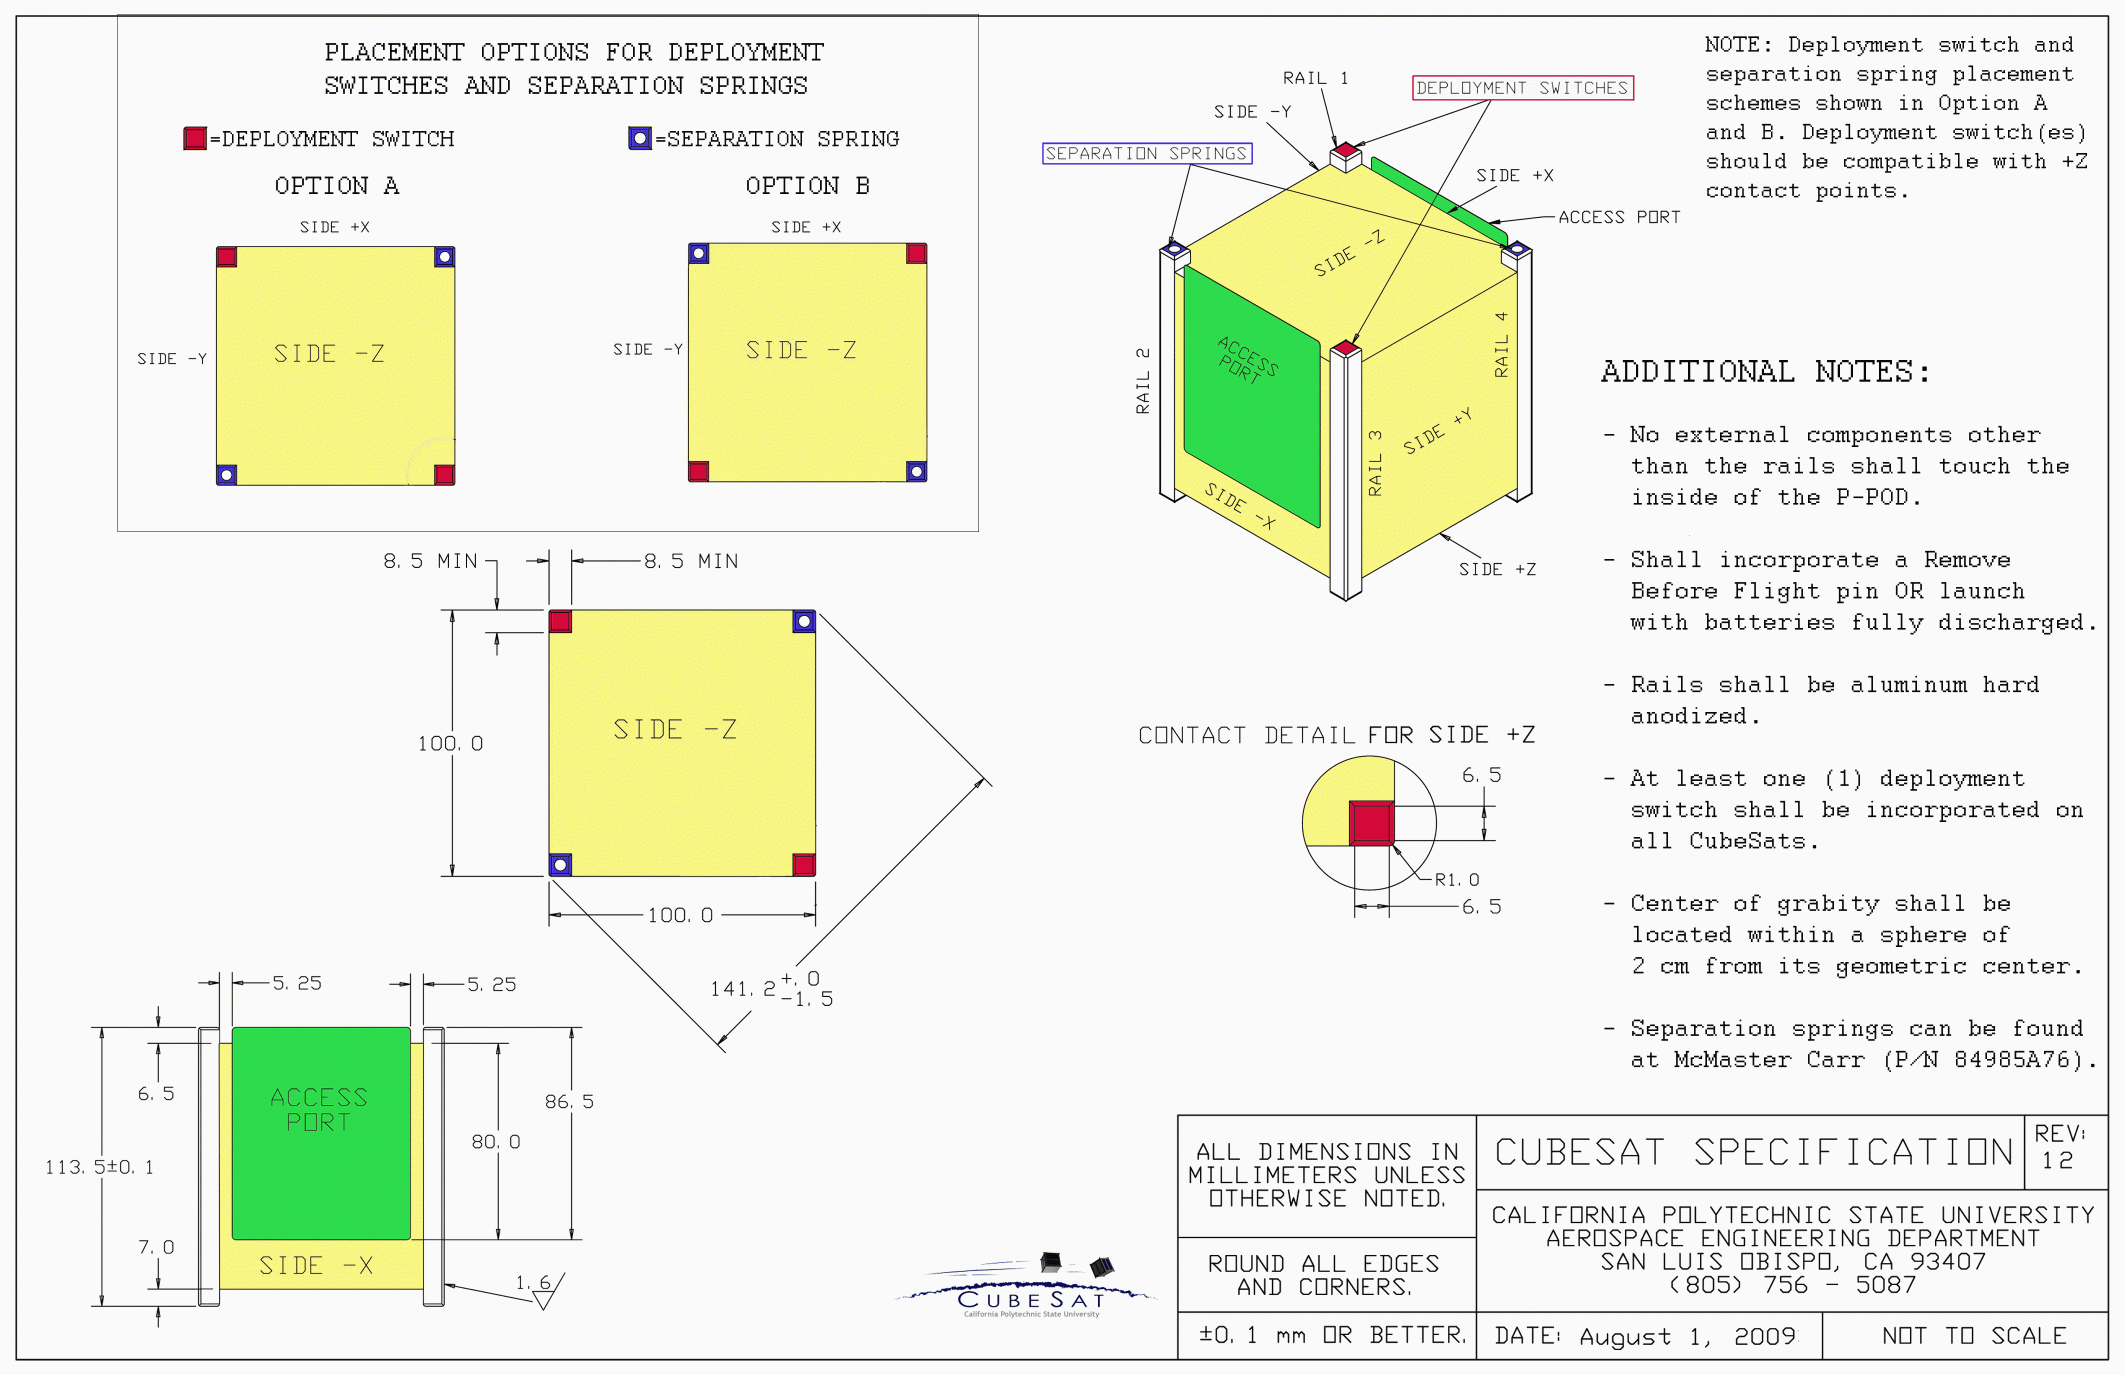
\includegraphics[scale=0.6]{./ANNEXES/images/CubeSatDesign}
\centering
\caption{Dimensions of a 1U CubeSat}
\cite{cubesatdimensions}
\label{epsschematics}
\end{figure}

\paragraph{}The two most interesting options that were considered when the structure had to be chosen are presented below.

\begin{longtable}{| l | c | c | }
\hline
\rowcolor[gray]{0.80}	\textbf{Brand and model} &  \textbf{Features}     & \textbf{Total price (\euro)}   \\
\hline
\endfirsthead

\rowcolor[gray]{0.85} \textbf{Structure} &  &  \\
	   ~ISIS 3U structure & \makecell{Low mass (304.3g) \\ Highly compatible \\ High temperature range} & 3900 \\
	   \hline
	   ~Gomspace GOMX-Platform & \makecell{High mass (1500g) \\ Comes fully equipped (basic systems) \\ High temperature range} & 11000 \\
	   \hline
\caption{Options studied for the structure}
\label{structureoptions}
\end{longtable}

\subsubsection{Thermal protection}
\paragraph{}The thermal protection system consists of various insulating materials that aim to protect the CubeSat from potential thermal shocks. Currently, the most used element as thermal protection in the aerospace industry is the multilayer insulation (MLI), a set of multiple thin insulation layers. The MLI fulfills all the requirements of this mission and its main objective is to reduce the heat generated by radiation, given that the heat generated by convection or conduction does not have such a high impact on the on-board systems.

\paragraph{} 
After a market study, \textit{Dunmore Aerospace} company has been chosen to provide us its MLI product. Specially, the product is the \textbf{Dunmore Aerospace Satkit} and it is made for small satellites for LEO and it will provide the CubeSat with the protection required during operation

\subsubsection{Study of the commercial available options and options chosen}
\paragraph{}A broad marked study is needed since all the options have to be considered. For this reason, and with the aim to show all the information and features of each system that has been considered in this section, the table \ref{structureoptions} is presented below.


\begin{longtable}{| l | c | c | }
\hline
\rowcolor[gray]{0.80}	\textbf{Brand and model} &  \textbf{Features}     & \textbf{Total price (\euro)}   \\
\hline
\endfirsthead

\rowcolor[gray]{0.85} \textbf{Structure} &  &  \\
	   ~ISIS 3U structure & \makecell{Low mass (304.3g) \\ Highly compatible \\ High temperature range} & 3900 \\
	   \hline
	   ~Gomspace GOMX-Platform & \makecell{High mass (1500g) \\ Comes fully equipped (basic systems) \\ High temperature range} & 11000 \\
	   \hline
\rowcolor[gray]{0.85} \textbf{Thermal protection} &  &  \\
	   ~Dunmore Aerospace Satkit & \makecell{Lightweight \\ Durability \\ Made for small satellites}& \textbf{TO REQUEST!} \\
	   \hline
	   ~Dupont Kapton Aircraft Thermal & \makecell{Lightweight \\ Durability \\ Non-flammable} & \textbf{TO REQUEST!} \\
	\hline

\caption{Options studied for the structure and thermal protection}
\label{structureoptions}
\end{longtable}

\paragraph{}Finally, the options chosen are presented in the table \ref{structurefinal}.

\begin{longtable}{| l | r | r | r | }
\hline
\rowcolor[gray]{0.80}	\textbf{System} &  \textbf{Brand and model}     & \textbf{Price per unit (\euro)} & \textbf{N. of units}  \\
\hline
\endfirsthead

	   ~3U Structure & ISIS & 3900 & 1 \\
	   \hline
	   ~Thermal Protection & Dunmore Satkit & TO REQUEST & 1\\
	\hline

\caption{Options chosen for the structure and thermal protection}
\label{structurefinal}
\end{longtable}
